\chapter{Flight Data}
For data analysis, the data of German flights was required. There is no open source datasets available for Germany flights so all this data had to be taken from scratch. There are numerous websites that do keep record of historical data of flights. But none of the free versions of the websites provided either the API or historical data for free. At the end, Flightradar24 was selected for their cheap Gold tier options which provided us last six months of historical flight data for each flight in the world. But first we also needed the actual flights for which we needed the records.

\section{List of all flights landing in Germany}
For getting the data from FlightRadar24, the first task was to create a list of flights that are landing in Germany from any airport in the world. Luckily, doing quick search on Flightradar24 we had a small list of 56 airports that are used for commercial and charter flights in Germany [EC]. The airports that just handled chartered flights were ignored for this dataset. As this was a small task and didn't require much time, this whole process was done manually. For each airport of Germany, we had all the flights which were landing on that airport. Each record was copied into an excel file, available on github, with the most important flight details. The records contained the origin airport, the destination airport, the standard arrival and departure of the flight, and most importantly, the flight ID and name of the airline. On completing the task we had about 3000 flights that came in from more than 200 cities in the world and landed in one of the 28 biggest airports in Germany.

\section{Plausible Sources for historical flight data}
Once we had details of all the flights landing in Germany, the next step was to get the historical data of at least 3 months for each flight in our list. As this was going to be a huge dataset that cannot be created/curated manually, the requirements for selecting data sources were defined as follows:
\begin{enumerate}
    \item The flight data source should have at least 3 months of historical data of flights, especially the actual departure, actual arrival and flight delay.
    \item The flight data source should preferably have a developer friendly API to automate the whole process of getting the data
    \item The API calls or subscription costs for the flight data source should be reasonable
\end{enumerate}

Based on the above mentioned criteria, the following flight data sources were evaluated. 
\subsection{Flightstats}
Flightstats keeps track of the flights across the world. They have a developer API but it is not easy to register. The user has to give specific domain where their data will be used, assure them there will be no commercial use and give details of what kind of data would be required. On making the request multiple times, our request was rejected. Soon a call was received from flightaware sales team that offered to provide the complete dataset as an excel file instead. The happiness of receiving the complete and clean data was shortlived though as the company asked for 2000€ for the dataset. Hence Flightstats was not considered anymore.

\subsection{Flightaware}
Flightaware is one of the biggest websites in the world providing live flight tracking across the globe. [EC] They have a very user friendly developer API which provides interface for REST requests. The developer key is provided free of cost. The free account of flightaware.com gives us historical records of 14 days only. At \$20 per month, the flight history provided is 5 months.[EC] But on further research, it was noted that  the historical data was just for display. Their API, FlightXML 3 doesn't provide making REST requests for historical data of a flight via API \url{[https://flightaware.com/commercial/flightxml/pricing_class.rvt}.
Hence this website was not selected

\subsection{Flightradar24}
Flightradar24 is one of the most famous sites on internet and even has android and iPhone apps that provide real time flight path and flight status. Even though the free account has just 14 days of historical data, the Gold tier, costing just 5 Euros, had flight history of 6 months. But the biggest issue in selecting Flightradar24 was that they have no developer friendly API to get flight stats. But being out of options, this site was selected for at least being more suitable than other websites analysed.

\section{Getting data}
Not having a API for getting flight history was an obstacle in collecting data but it could be overcome by scraping the flight data instead. As we could see last 6 months of flight data on the webpage.
Even though many websites specifically consider web scraping illegal, flightradar24 only rejects web-scraping of data if that data is to be used commercially[EC]. Hence this website being a college project, doesn't fit under the commercial category.

\subsection{scraping}
Web scraping is basically looking into the source code of a webpage and saving the data you require[EC]. As we already had the flight ID of all the flights in Germany, the list for all webpages which would have to scraped was created using the URL template \url{https://www.flightradar24.com/data/flights/<flight_id>/}. 
Once we had all the web-URLs to be scraped, the actual scraping was started. \\As the whole website was to be created in Python so  the scraping was also done in Python.Python has a very handy utility that provides a very easy to use library for web scraping called Scrapy. 
In the most basic sense, we get the whole webpage, and then save the desired elements of the URL in JSON format. The important variables for us were 'From', 'To', flight time, STD, AD, SA, AA. All of this data was saved in a csv file.
 

\section{Data Variables}
All the data we received from scraping was saved in a csv file.
The total records we saved were about 385,000 but many of the observations were missing important variables. In this section we go through each variable and then later on dwell into the cleaning of data so that it's suitable for analysis.
\begin{enumerate}
    \item {Departure Airport}
    \\Origin Airport of the flight. This value can be of any airport in the world that has a direct flight to a German airport
    \item {Arrival Airport}
    \\Destination airport of the flight. It will always be one of the German airports
    \item {Standard Arrival}
    \\The fixed arrival time of a flight time based on the flight schedule.
    \item {Actual Arrival}
    \\The actual arrival of the flight, that might be earlier or most probably at or after the standard arrival of the flight
    \item {Standard Departure}
    \\The fixed departure time of a flight time based on the flight schedule.
    \item {Actual Departure}
    \\The actual departure of the flight, that might be earlier or most probably at or after the standard departure of the flight
    \item {Airline}
    \\The flight company
    \item {Flight ID}
    \\The The flight ID is a unique number provided by International Air Transport Organisation to each flight.
    \item {Aircraft}
    \\The type of aircraft for the flight
\end{enumerate}

\section{Data Cleanup and missing values substitution}
On opening the csv file with all the stored data, it could be noted that a lot of data had some missing values. A lot of data we had was  repetitive data, for ex arrival and destination airports stay same for the flight no matter the date of flight. But some of the data like flight time would change everyday. Hence different strategies were created for cleaning missing values for each variable.
Excel was selected for data cleanup due to its ease of use and data visualisation capabilities

\subsection{Departure Airport}
Departure Airport stays constant for each Flight ID. Many of the flight IDs had different airports on different dates, and some were missing the value. This was rectified for each of the 3000 different flights.

\subsection{Arrival Airport}
The same strategy was applied to Arrival airport for cleanup as we used for Departure Airport. But this variable had couple of more problems that needed different fix:
\begin{enumerate}
    \item Flight diverted
    \\Arrival airport too remains constant for each Flight ID except in case the flight is diverted. This was a special case and only happened nine times in our dataset. All these entries were removed. \item Connecting Flights
    \\There are many indirect flight that connect to German airports. For sake of simplicity, it was decided to keep only flight lading in Germany. For ex, if a flight flew from Delhi to Moscow, and then from Moscow to Frankfurt, only flight that came from Moscow was considered and rest were discarded. 
\end{enumerate} 

\subsection{Standard Arrival}
The Standard Arrival of a flight does not necessarily stay the same all year. For ex., it changes on the basis of daylight savings or even as a business decision by an airport or Airline. Hence instead of changing all values of standard departure same for complete history of a flight, the values were copied from the upper or lower cell in the data belonging to the same flight. 

\subsection{Standard Departure}
The same strategy as for Standard Arrival was used for cleaning up Standard Departure too.

\subsection{Actual Arrival}
Arguably the most important variable that we have in our dataset. The actual flight delay will be calculated using this variable. Any row that doesn't has this value is removed from the dataset.

\subsection{Actual Departure}
Any values that were missing from actual departure, were assumed to be the same as standard departure as the variable was of not much importance to us.
\subsection{Airline}
The airline was corrected on the basis of the upper or lower cells in the dataset. 

\subsection{Flight ID}
Even though an important variable, it's not at all required for our data analysis. The variable was left as is.

\subsection{Aircraft}
For cleaning the missing data in Aircraft, it was assumed that a flight uses same aircraft unless a pattern is noticed where each subsequent flight uses a different aircraft.

\subsection{Flight duration}
Another very important variable in our dataset. And missing value was calculated by subtracting Actual departure from Actual Arrival. All the values were also converted into seconds instead of keeping them in Time format.

\section{Adding new variables}
After cleaning the dataset, we decided to add new variables to the dataset which would hopefully make the predictions better aligned to our end goal

\subsection{Flight delay bins}
Out insurance rates will vary based on our flight delay prediction. To ease this process and give customer a better perspective about the insurance payout, we create 4 different categories of flight Instead of using the exact time of delays. 
\begin{enumerate}
    \item 0 if flight is on time or less than 15 minutes late
    \item 1 if flight is 15 or minutes but less than an hour late
    \item 2 if flight is more than 15 minutes but less than an hour late
    \item 3 if flight is an hour or more late
\end{enumerate}

\subsection{Weekend}
A simple variable. Using Weekday formula in excel, we create a binary variable which is true if the flight is on weekends.

\subsection{Time Blocks}
Instead of using exact arrival time of our flight, we create multiple time blocks of 2 hours so that this variable can be used as factor for our classification algorithms. A flight at 8:30 in the morning was classified in block 8 and flight at 15:30 is classified in block 16.

\section{Reducing Levels}
One problem that we face in classification algorithms when analysing such a big dataset is number of categories of each variable. We have more than 50 airlines and 80 aircraft in our dataset. Algorithms in R like random forest don't accept more than 32 categories.[EC] Boosting algorithms like XGBoost on the other hand require indicator columns instead of categorical variable[EC]. Hence each column with n categories is converted to n columns. This makes the dataset too large. Reducing levels will help in this scenario too.

\subsection{Airline}
We had 67 different airlines in our dataset with Lufthansa being the most popular with 124940 flight records. We can see in the figure  that we have many airlines with insignificant number of flights. 
%insert image
Hence we combine the airlines with lowest number of flights in a new airline category called other\_airline

\begin{figure}[ht]
    \centering
    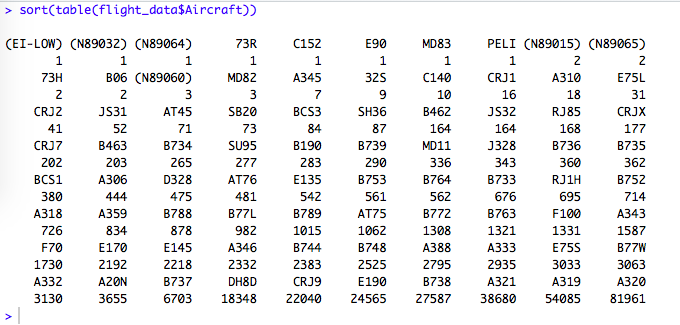
\includegraphics[width=\textwidth]{Figures/Aircraft_orig_levels.png}
    \caption{Reduced categories of Airlines with number of airline}
    \label{fig:airline2}
\end{figure}

\subsection{Aircraft}
We had about 80 different kind of aircraft in our dataset, with Airbus A320 being the most common choice, with over 81000 flights. We can see in the figure \ref{fig:aircraft1} that we have many aircraft with insignificant number of flights.

\begin{figure}[ht]
    \centering
    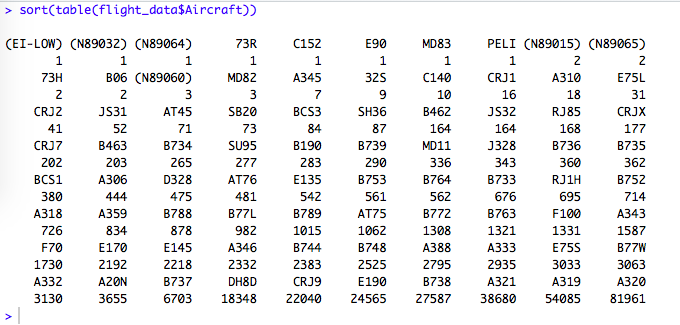
\includegraphics[width=\textwidth]{Figures/Aircraft_orig_levels.png}
    \caption{Original categories of Aircraft with number of flights}
    \label{fig:aircraft1}
\end{figure}

We combine all the aircraft with the lowest number of variables in a new value called other\_aircraft, as seen in figure \ref{fig:aircraft2}.

\begin{figure}[ht]
    \centering
    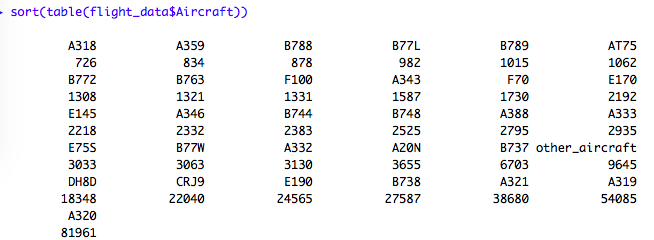
\includegraphics[width=\textwidth]{Figures/Aircraft_reduced_levels.png}
    \caption{Reduced categories of Aircraft with number of flights}
    \label{fig:aircraft2}
\end{figure}

\subsection{Departure Airport}
The departure airport has 287 different departure airports from all over the world. Many of the airports have non-insignificant number of flights so converting a majority of flights to a single category would have been counter-productive. Hence we left the variable as is to measure if this variable is any important to our prediction or could be left out.

\section{End result - dataset}

After cleaning the data, substituting the missing values, reducing the number of levels and adding new variables to help in prediction, the summary of the dataset is as seen in figure \ref{fig:summary_flights}:

\begin{figure}[ht]
    \centering
    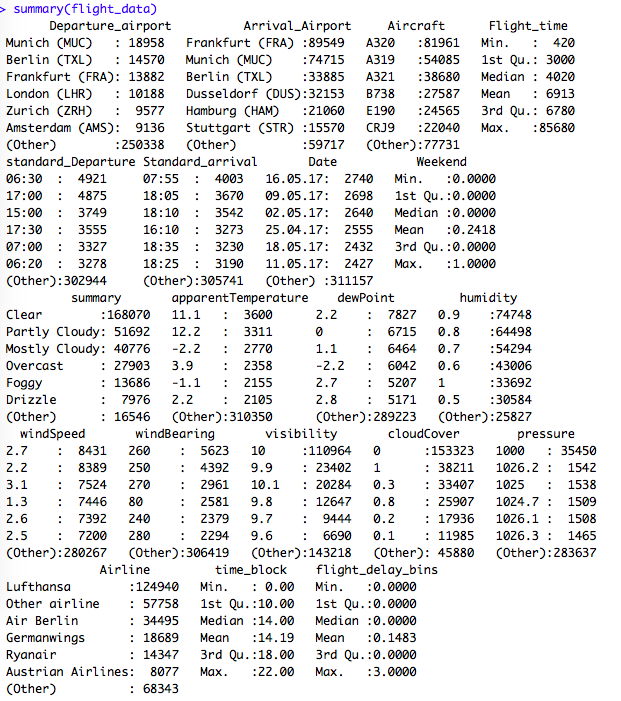
\includegraphics[width=\textwidth]{Figures/summary_flight_data.png}
    \caption{Final summary of our flight dataset}
    \label{fig:summary_flights}
\end{figure}